\documentclass[border=3pt]{standalone}
\usepackage{circuitikz}
\usetikzlibrary{positioning,calc}
\ctikzset{logic ports=ieee, logic ports/scale=0.9}
\begin{document}
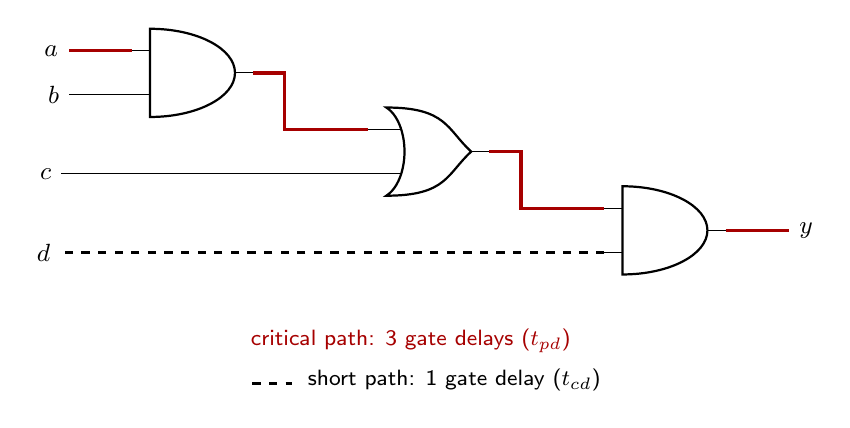
\begin{tikzpicture}[font=\sffamily\small]
  \node[and port] (g1) at (0,0) {};
  \node[or port]  (g2) at (3,-1.0) {};
  \node[and port] (g3) at (6,-2.0) {};
  % critical path: a -> g1 -> g2 -> g3 -> y (3 gate delays)
  \draw[very thick, red!65!black] (g1.in 1) -- ++(-0.8,0) node[left, black]{$a$};
  \draw (g1.in 2) -- ++(-0.8,0) node[left]{$b$};
  \draw[very thick, red!65!black] (g1.out) -- ++(0.4,0) |- (g2.in 1);
  \draw (g2.in 2) -- ++(-3.9,0) node[left]{$c$};
  \draw[very thick, red!65!black] (g2.out) -- ++(0.4,0) |- (g3.in 1);
  % short path: d -> g3 only (1 gate delay)
  \draw[very thick, dashed] (g3.in 2) -- ++(-6.9,0) node[left]{$d$};
  \draw[very thick, red!65!black] (g3.out) -- ++(0.8,0) node[right, black]{$y$};
  % legend
  \node[anchor=west, red!65!black] at (0,-3.4) {\footnotesize critical path: 3 gate delays ($t_{pd}$)};
  \node[anchor=west] at (0,-3.9) {\footnotesize \tikz{\draw[very thick, dashed] (0,0)--(0.5,0);}\; short path: 1 gate delay ($t_{cd}$)};
\end{tikzpicture}
\end{document}
